\section{MOTIVATING EXAMPLE}
\label{sec:motivate}
\begin{figure*}[!ht]
    \centering
    \subfigure[Example]{
    	\label{fig:sub:example}
        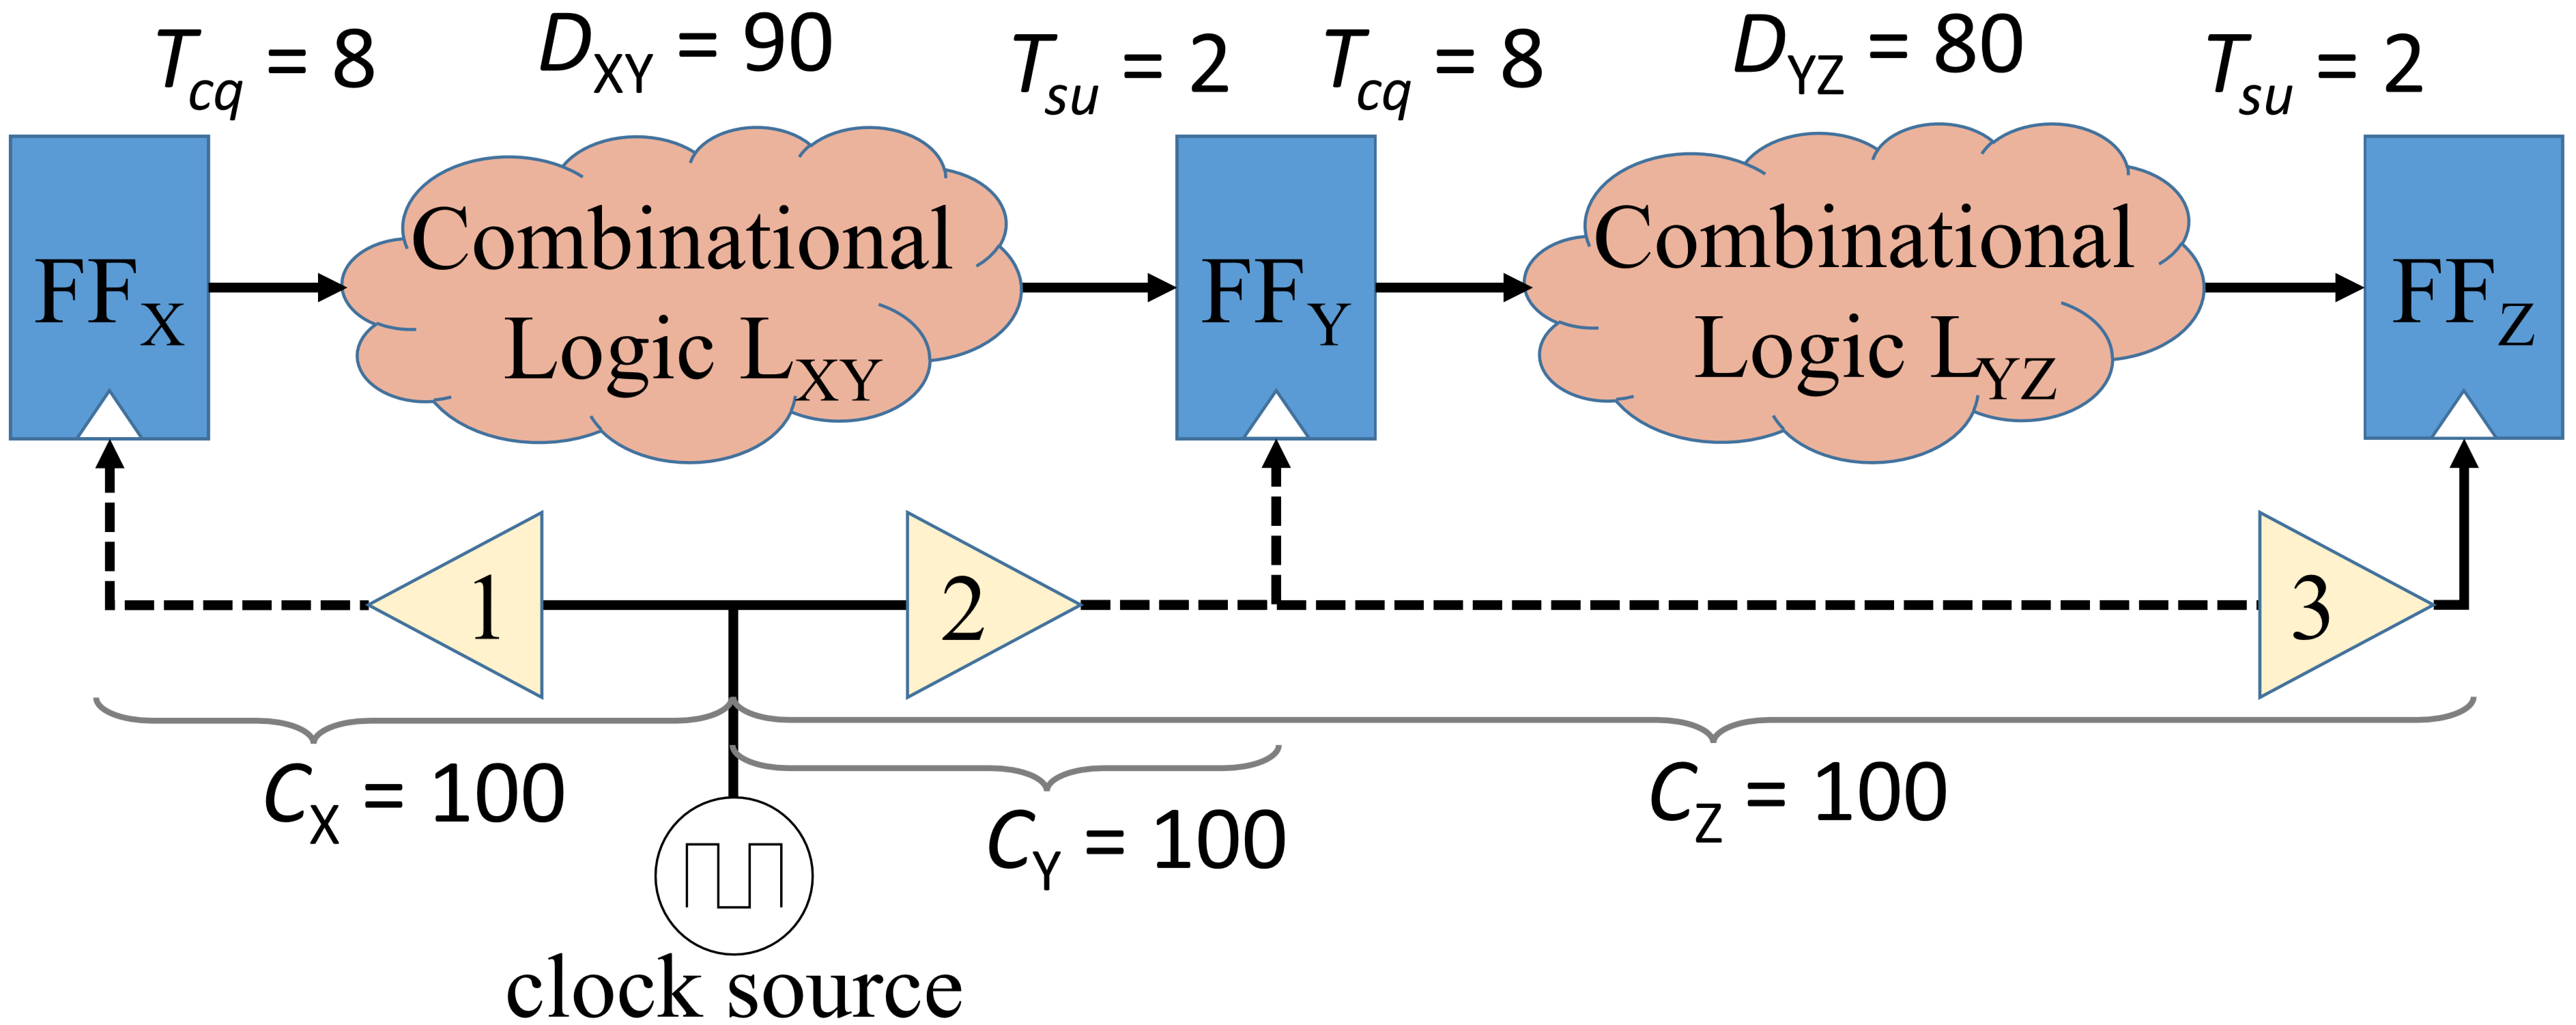
\includegraphics[width=0.9\columnwidth]{Motivating_example.png}
    }
    \hspace{1.6cm}
    \subfigure[Notations]{
    	\label{fig:sub:notations}
        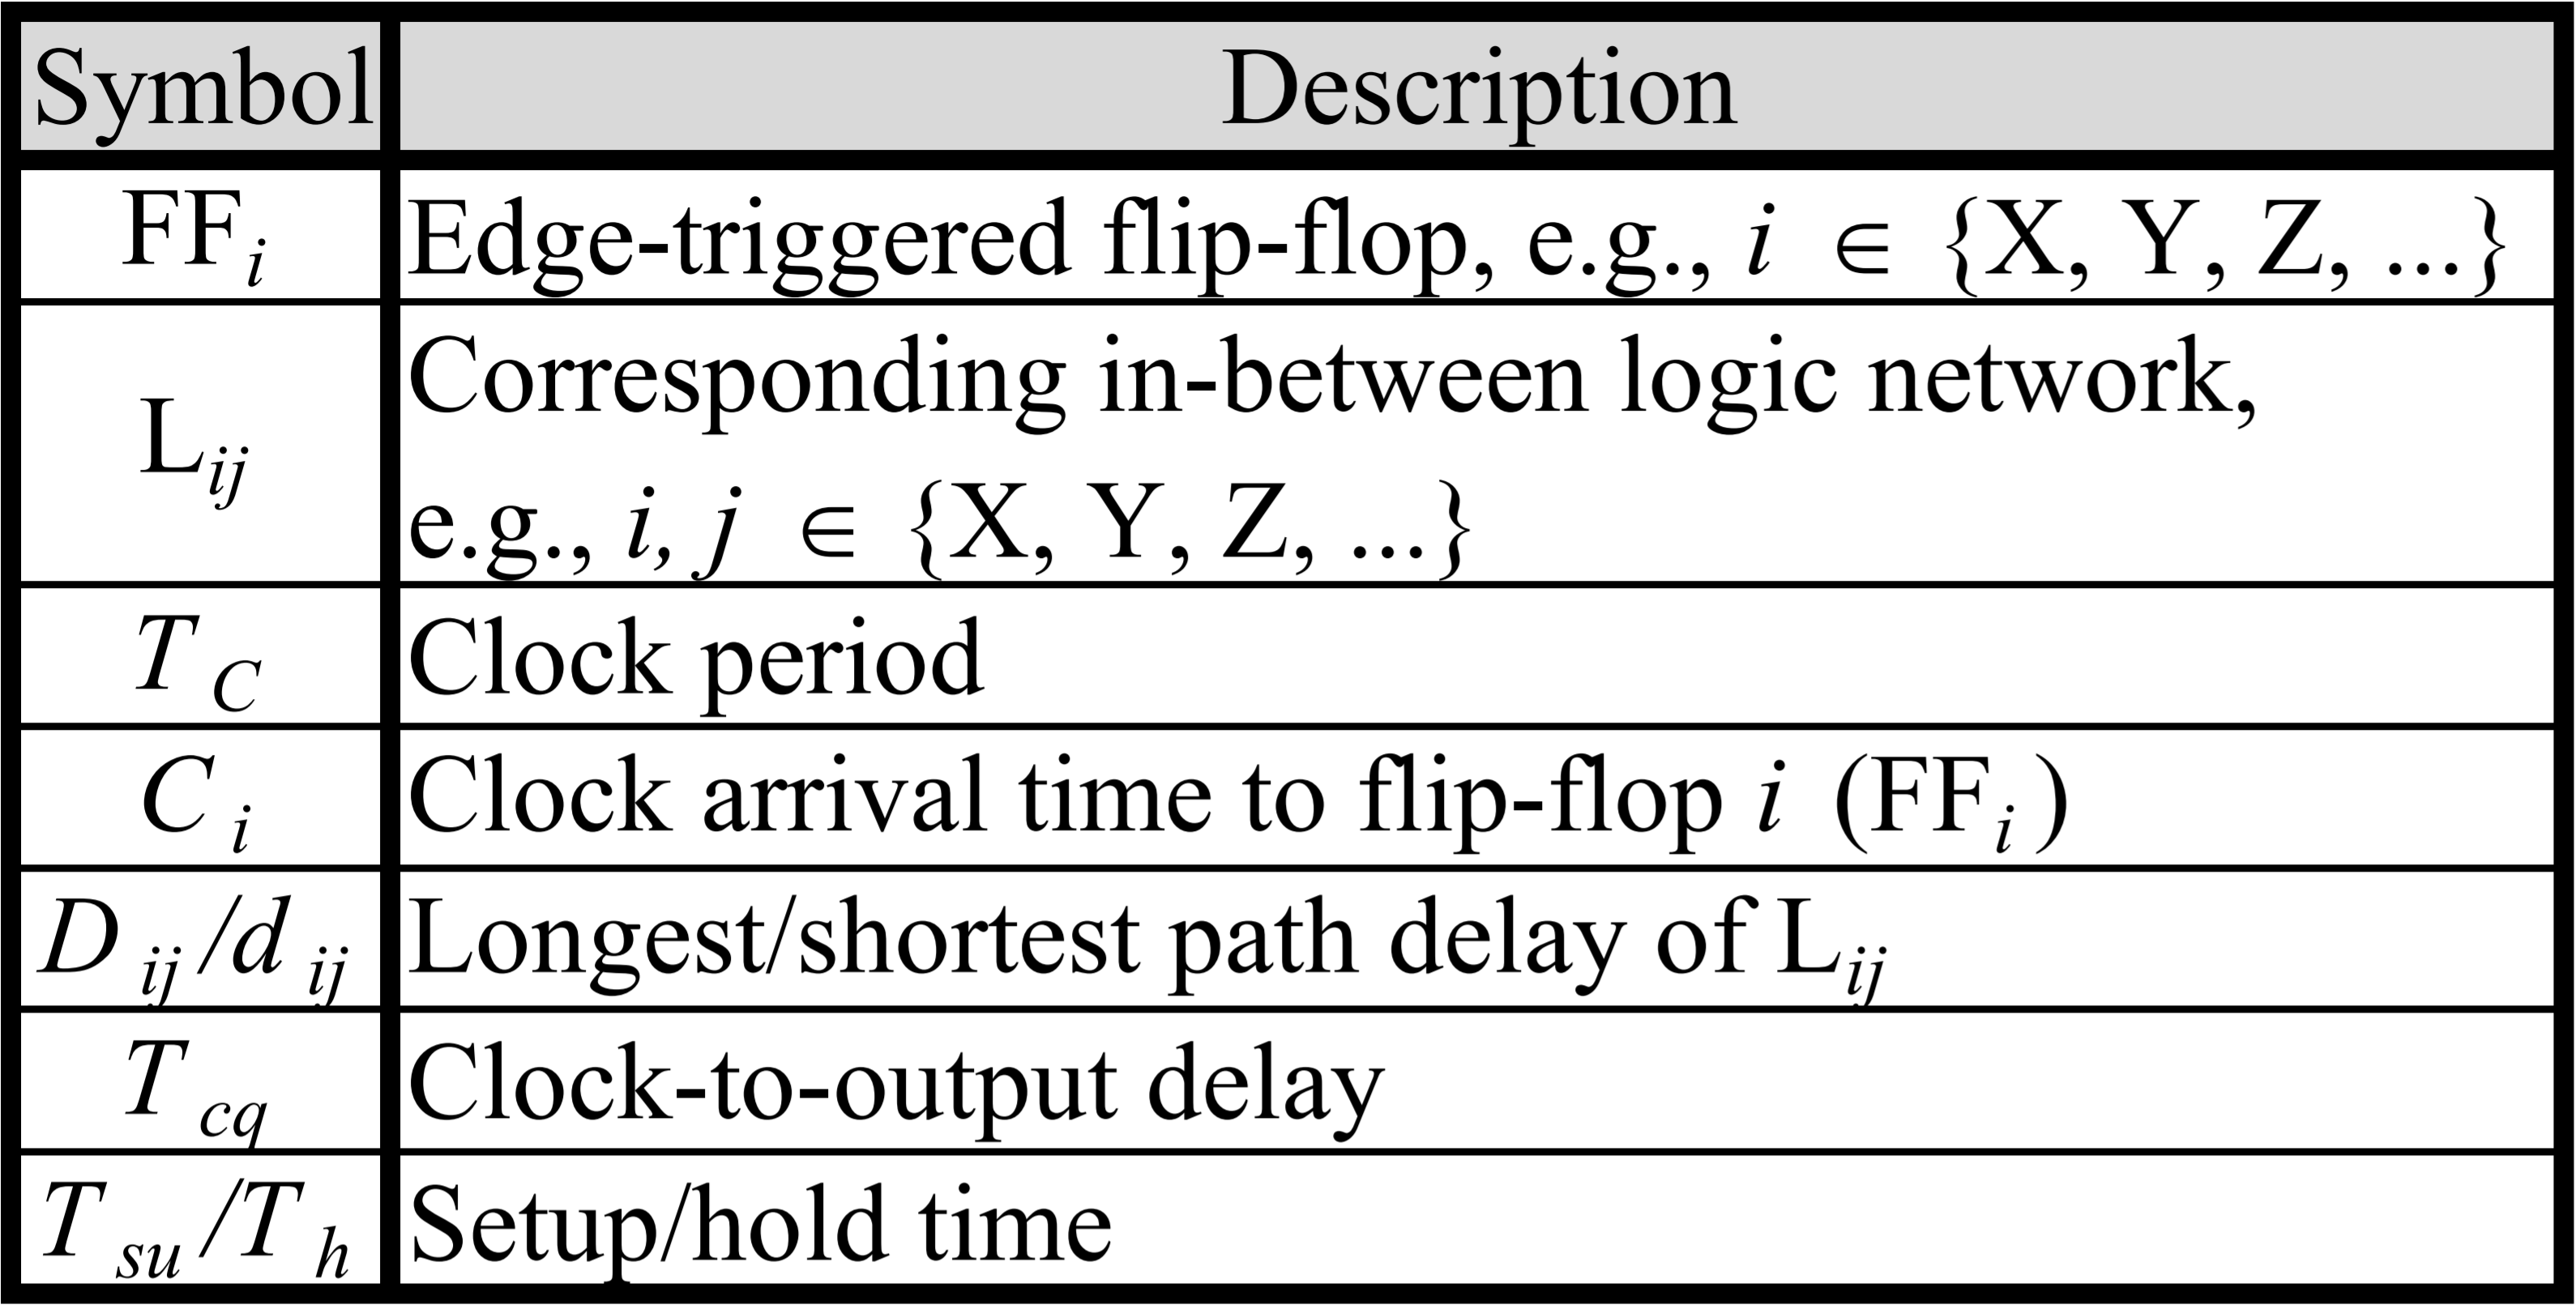
\includegraphics[width=0.8\columnwidth]{Notations.png}
    }
    \caption{Illustrative example and notations for the proposed framework based on DCC deployment/insertion}
    \label{fig:en}
\end{figure*}


%DATE 2018
This section introduces two illustrative examples which motivates our idea of making clock skew useful, based on the two methodologies: ($i$) Manipulate the aging behaviors of clock paths ()and  Consider the circuit in Figure~\ref{fig:sub:example} where \ce{FF_X}, \ce{FF_Y} and \ce{FF_Z} are three edge-triggered flip-flops, and \ce{L_{XY}} and \ce{L_{YZ}} are the corresponding in-between logic networks. Other notations to be used later are listed in Figure~\ref{fig:sub:notations}.

For each pair of flip-flops (e.g., \ce{FF_i} and \ce{FF_j}) between which there exists at least one logic path from \ce{FF_i} to \ce{FF_j}, the following setup-time (Equation (\ref{eq:tsu})) and hold-time (Equation (\ref{eq:th})) constraints need to be satisfied:
\begin{equation}
	\mbox{\fontsize{9}{9.6} $C_i+T_{cq}+D_{ij}+T_{su}<C_j+T_c$}
	\label{eq:tsu}
\end{equation}
\begin{equation}
	\mbox{\fontsize{9}{9.6} $C_i+T_{cq}+d_{ij}<C_j+T_h$}
	\label{eq:th}
\end{equation}

Assume that, at year 10, $D_{ij}$ is degraded by 15\%, and both $T_{cq}$ and $T_{su}$ increase by 20\%. By using the predictive model presented in~\cite{wang2010impact},~\cite{wang2007efficient}, we can accurately derive the aging of $C_i$ and $C_j$ due to the regularity and predictability of a typical clock waveform of 50\% duty cycle. In the process technology used (TSMC 45nm GP standard cell series), $C_i$ and $C_j$ are degraded by 13\% under 10-year BTI, i.e., $C_i$ and $C_j$ become 1.13X larger.

To be aging-aware for the example circuit in Figure~\ref{fig:sub:example}, we have to consider aforementioned aging factors in the setup-time constraints on \ce{L_{XY}} and \ce{L_{YZ}}:
\begin{equation}
\mbox{\fontsize{9}{9.6}\selectfont \ce{L_{XY}}:\quad$\textbf{1.13}C_X+1.2T_{cq}+1.15D_{XY}+1.2T_{su}<\textbf{1.13}C_Y+T_c$} 
\label{eq:lxy}
\end{equation}
\begin{equation}
\mbox{\fontsize{9}{9.6}\selectfont \ce{L_{YZ}}:$\quad\textbf{1.13}C_Y+1.2T_{cq}+1.15D_{YZ}+1.2T_{su}<\textbf{1.13}C_Z+T_c$} 
\label{eq:lyz}
\end{equation}
where $C_X$ = $C_Y$ = $C_Z$ = 100, $T_{cq}$ = 8, $T_{su}$ = 2, $D_{XY}$ = 90 and $D_{YZ}$ = 80, as shown in Figure~\ref{fig:sub:example}.
\begin{flushleft}
By re-arranging Equations (\ref{eq:lxy}) and (\ref{eq:lyz}):
\begin{flalign*}
\hspace{1.2em}\ce{L_{XY}}: T_c &> 115.5 &\\
\hspace{1.2em}\ce{L_{YZ}}: T_c &> 104
\end{flalign*}
\end {flushleft}
Therefore, the clock period needs to be larger than 115.5 (dominated by \ce{L_{XY}}) to ensure no setup-time violation over a required lifespan of 10 years. For brevity, we omit the discussion on hold-time constraints, which in our work are actually formulated to ensure no existence of racing due to short paths.

%Example 1
%\subsection{Example 1: Aging Manipulation on Clock Network}
%\label{sec:motivate:exp1}
To minimize required $T_c$ under aging, we use \textit{duty-cycle converter} (DCC) to manipulate the aging rates of clock branches. We insert one 20\% DCC at the input of buffer 1, and another 80\% DCC at the input of buffer 2. The 20\% (80\%) DCC can decrease (increase) the stress times of downstream clock buffers by converting the clock duty cycle to 20\% (80\%), from a typical duty cycle of 50\%. Therefore, 20\% DCC can mitigate/decelerate the aging of $C_X$ and 80\% DCC can aggravate/accelerate the aging of $C_Y$. In the case of no DCC, $C_X$ and $C_Y$ are degraded by 13\% under 10-year BTI in TSMC 45nm GP standard cell series, while 20\% and 80\% DCCs will degrade $C_X$ and $C_Y$ by 9\% and 16\%, respectively, assuming that the clock paths from the clock source to \ce{FF_X} and \ce{FF_Y} are disjoint.

Consider the new aging factors (due to effects of various clock duty cycles) in the setup-time constraints on \ce{L_{XY}} and \ce{L_{YZ}}:
\begin{equation}
\mbox{\fontsize{9}{9.6}\selectfont \ce{L_{XY}}:\quad$\textbf{1.09}C_X+1.2T_{cq}+1.15D_{XY}+1.2T_{su}<\textbf{1.16}C_Y+T_c$} 
\label{eq:lxy2}
\end{equation}
\begin{equation}
\centering
\mbox{\fontsize{9}{9.6}\selectfont \ce{L_{YZ}}:\quad$\textbf{1.16}C_Y+1.2T_{cq}+1.15D_{YZ}+1.2T_{su}<\textbf{1.16}C_Z+T_c$} 
\label{eq:lyz2}
\end{equation}
By re-arranging Equations (\ref{eq:lxy2}) and (\ref{eq:lyz2}):
\begin{flalign*}
\hspace{1.2em}\ce{L_{XY}}: T_c &> 108.5 &\\
\hspace{1.2em}\ce{L_{YZ}}: T_c &> 104
\end{flalign*}
As it can be seen, we can reduce the required $T_c$ from 115.5 to 108.5 (dominated by \ce{L_{XY}} still), by adding two DCCs in the existing synthesized clock tree to create aging-induced clock skews. The skew for \ce{L_{XY}} (between \ce{FF_X} and \ce{FF_Y}), quantified as 1.16$C_Y$ minus 1.09$C_X$, is useful/beneficial and accounts for the reduction of required $T_c$. A certain level of aging tolerance is thus achieved because aging-induced performance degradation of $D_{XY}$ (plus $T_{cq}$ and $T_{su}$ actually) can be tolerated, by exploring such useful aging-induced clock skews.

\begin{comment} %TVA, DCC are equal
\subsection{Example 2: V\textsubscript{th} Assignment and Aging Manipulation on Clock Network}
\label{sec:motivate:exp2}
In the example, the two approaches, V\textsubscript{th} assignment and aging manipulation, are both applied to further optimize/reduce required $T_c$. We let the DCC deployment same with that in the first example, i.e., 20\% DCC and 80\% DCC are inserted at the inputs of buffer 1 and buffer 2, respectively. Moreover, a \textit{technology leader} is inserted at the input of buffer 2. Here, \textit{technology leader} denotes that, the technology of downstream (toward terminals/flip-flops) clock buffers are replaced with new technology, such that the V\textsubscript{th} of the buffers are changed. Note that, the so-called downstream clock buffers are those between technology leader and terminals/flip-flops. For instance, when one technology leader is inserted at the input of buffer 2, the downstream buffers are those in the intervals from buffer 2 to \ce{FF_x} and  to \ce{FF_y}, which also include buffer 2 and buffer 3, but exclude flip-flops. Therefore, we can find that, for the clock buffers, which are in the intervals from buffer 2 to \ce{FF_x} and  to \ce{FF_y}, their technology is replaced with the new counterpart. Note that, in the example, we consider one type of new technology: HTV (High Threshold Voltage or High-V\textsubscript{th}) technology. Thus, the associated technology leader is named \textit{HTV leader}, which assigns high-V\textsubscript{th} to the downstream clock buffers. To include the aging rates of HTV buffers (clock buffers with high-V\textsubscript{th}) in the setup-time constraint, we assume that, the fresh delay of HTV buffer is 1.2X longer than that of nominal buffer, and aging rates of HTV buffer, with the duty cycle of 20\%, 40\%, 50\% and 80\%, are 0.5\%, 4.1\%, 5.4\% and 8.2\%, respectively. Note that, the aging rates of HTV buffer are lower than those of nominal buffer, because the higher/lower V\textsubscript{th} leads to lower/higher aging rates. Consider the new aging factors in the setup-time constraints on \ce{L_{XY}} and \ce{L_{YZ}}:
\begin{equation}
	\mbox{\fontsize{9}{9.6}\selectfont \ce{L_{XY}}:\quad$\textbf{1.09}C_X+1.2T_{cq}+1.15D_{XY}+1.2T_{su}<\textbf{(1.2+0.08)}C_Y+T_c$} 
	\label{eq:lxy2}
\end{equation}
\begin{equation}
	\centering
	\mbox{\fontsize{9}{9.6}\selectfont \ce{L_{YZ}}:\quad$\textbf{(1.2+0.08)}C_Y+1.2T_{cq}+1.15D_{YZ}+1.2T_{su}<\textbf{(1.2+0.08)}C_Z+T_c$} 
	\label{eq:lyz2}
\end{equation}
By re-arranging Equations (\ref{eq:lxy2}) and (\ref{eq:lyz2}):
\begin{flalign*}
	\hspace{1.2em}\ce{L_{XY}}: T_c &> 96.5 &\\
	\hspace{1.2em}\ce{L_{YZ}}: T_c &> 104
\end{flalign*}

Apparently, the required $T_c$ is further reduced/optimized from 108.5 to 104 (dominated by \ce{L_{YZ}} rather than \ce{L_{XY}} in the first example), by inserting two DCCs and one HTV leader in the existing synthesized clock network. Note that, there exists a difference between DCC and HTV leader. DCC is a physical gate; however, HTV leader is conceptually an imaginary location, from which we begin manipulating the technology of clock buffers toward flip-flops. As it can be seen, when the two approaches, V\textsubscript{th} assignment and aging manipulation  (by DCC insertion) , are applied together in the second example, the skew for \ce{L_{XY}}, which equals 1.28$C_Y$ minus 1.09$C_X$, is larger than that in the first example. Therefore, the new skew for \ce{L_{XY}} is more useful/beneficial and accounts for the better optimization of required $T_c$. 
Additionally, when it comes to the timing-borrowing mechanism of the two examples, there exists a difference: 1) The timing-borrowing mechanism, in the first example, is achieved by the aging-induced clock skew, caused by manipulating the duty-cycle delivered to flip-flops. 2) In the second example, the timing-borrowing mechanism is based on aging-induced clock skew and \textit{tech-induced} clock skew, which is caused by manipulating the technology of clock buffers, i.e., re-assign the V\textsubscript{th} of clock buffers. 
\end{comment}

One may note that \textit{clock skew scheduling} (CSS)~\cite{fishburn1990clock}, which derives unequal delays for all clock branches prior to \textit{clock tree synthesis} (CTS), can also optimize a circuit for aging tolerance. However, the optimization potential of general CSS is limited since it is difficult to precisely implement a wide range of clock delays during~\cite{li2011optimal}.

In contrast, post-CTS clock skew scheduling based on buffer insertion is another option. We will demonstrate that, if buffer insertion is employed to match our optimization results based on DCC insertion, the number of inserted buffers is usually much larger than the number of inserted DCCs. Also, as described later in Section~\ref{subsec:tpc}, the overhead of a single DCC can be diminished by integrating a DCC with its downstream buffer, which further reveals the cost effectiveness of our proposed DCC-based framework.

\subsection{Aging Prediction Model}
\label{subsec:apm}
Before discussing the proposed framework, we briefly introduce the aging (BTI degradation) model for logic gates/networks~\cite{wang2010impact},~\cite{wang2007efficient} used in our paper. This model enables us to analyze the long-term behavior of BTI-induced MOSFET degradation, with both aging and recovery mechanisms taken into account. First, the degradation of threshold voltage at a given time $t$ can be predicted as:
\begin{equation}
\label{eq:dtv}
\Delta V_{th}=\left(\frac{\sqrt{K_v^2 \cdot T_{clk} \cdot \alpha}}{1-\beta_t^{1/_{2n}}}\right)^{2n}
\end{equation}
where $K_v$ is a function of temperature, electrical field, and carrier concentration, $\alpha$ is the stress probability, and $n$ is the time exponential constant, 0.2 for the used technology. The detailed explanation of each parameter can be found in~\cite{wang2010impact}.

Next, the authors of~\cite{wang2007efficient} simplify this predictive model to be:
\begin{equation}
\label{eq:dtv2}
\Delta V_{th}=b\cdot  \alpha^n \cdot t^n = b \cdot \left(\alpha \cdot t \right)^n
\end{equation}
where $b = 3.9 \times 10^{-3} V \cdot s^{-1/_5}$.

Finally, the rising/falling propagation delay of a gate through the degraded P-type/N-type MOSFET can be derived as a first-order approximation:
\begin{equation}
\label{eq:pd}
\tau_p^\prime = \tau_p + a \cdot \left(\alpha \cdot  t\right)^n
\end{equation}
where $\tau_p$ is the intrinsic delay of the gate without BTI degradation and $a$ is a constant.

We apply Equation (\ref{eq:pd}) to calculate the delay of each gate under BTI, and further estimate the performance of a logic circuit. The coefficient $a$ in Equation (\ref{eq:pd}) for each gate type and each input pin is extracted by fitting HSPICE simulation results in 45nm, Predictive Technology Model (PTM). The simplified long-term model successfully predicts the MOSFET degradation, with less than 5\% loss of accuracy against cycle-by-cycle simulations~\cite{wang2010impact}.
